\documentclass[11pt,peerreview]{IEEEtran}

%\usepackage{biblatex}
%ARABIC SECTIONS
\renewcommand\thesection{\arabic{section}}
\renewcommand\thesubsection{\thesection.\arabic{subsection}}
\renewcommand\thesubsubsection{\thesubsection.\arabic{subsubsection}}

\renewcommand\thesectiondis{\arabic{section}}
\renewcommand\thesubsectiondis{\thesectiondis.\arabic{subsection}}
\renewcommand\thesubsubsectiondis{\thesubsectiondis.\arabic{subsubsection}}

\usepackage{caption}
\raggedbottom
\usepackage{mathtools}
\usepackage{graphicx}
\usepackage{color}
\usepackage[margin=1in]{geometry}
\usepackage{amsfonts,amsmath,amssymb}
\usepackage[none]{hyphenat}
\usepackage[nottoc,notlot,notlof]{tocbibind}
\usepackage{fixltx2e}
\usepackage{siunitx}

%Clikcable Links
\usepackage{hyperref}
\hypersetup{
    colorlinks,
    citecolor=black,
    filecolor=black,
    linkcolor=black,
    urlcolor=blue
} 
 
%For placing the logo properly.
%Probably not the best way to do it
\newlength{\PictHOffset}
\newlength{\PictVOffset}
\setlength{\PictHOffset}{1in}
\addtolength{\PictHOffset}{\hoffset}
\addtolength{\PictHOffset}{\oddsidemargin}
 
\setlength{\PictVOffset}{0in}
\addtolength{\PictVOffset}{\voffset}
\addtolength{\PictVOffset}{\topmargin}
\addtolength{\PictVOffset}{\headheight}
\addtolength{\PictVOffset}{\headsep}
\addtolength{\PictVOffset}{\topskip}
\addtolength{\PictVOffset}{-0.25\paperheight}

\usepackage{floatrow}
\floatsetup[table]{capposition=top}
\pagenumbering{Roman}
\parindent 0ex
\setlength{\parskip}{1em}
\renewcommand{\baselinestretch}{1.5}

\newcommand\tab[1][1cm]{\hspace*{#1}}
 
\begin{document}
 
\begin{titlepage}
    \noindent\hspace*{-\PictHOffset}%
    % Uncomment next line and replace XXX by your graphics file
    \raisebox{\PictVOffset}[100pt][0pt]{\makebox[0pt][l]{%
     
\includegraphics[width=\paperwidth,height=0.45\paperheight]{pukke.png}}}

 
    \begin{center}
    	\vfill
        \Huge {\textbf{Project Title}}
    	\vfill
        \LARGE{\textbf{A. T. Coetzee}}
        \vfill
        \huge{\textbf{Type of document}}
        \vfill
    \end{center}
    \textbf{Supervisor: \tab[2cm] Prof. Smart Man}\\
    \textbf{Date: \tab[3cm] \today}\\
    \textbf{Student Number: \tab[1cm]  123456789}\\
    \vfill
\end{titlepage}

%regular prerequisites for a document, contents, tables, figures

\pagebreak

\begin{abstract}
Sample abstract. You can reference appendices like so, (SEE APPENDIX \ref{AppRange}) 
\end{abstract}

\pagebreak

\tableofcontents

\listoffigures

\listoftables

\pagebreak
%document start
\pagenumbering{arabic}

\setcounter{page}{1}

\section{Design Requirement}
With the aid of a cellphone's accelerometer, design a scale capable of measuring an object's mass.

\section{Theoretical Design}
\subsection{Background}
Newton's Second Law is given by
\begin{equation}\label{eq:Newton2}
    \mathbf{F} = m\mathbf{a},
\end{equation} where $\mathbf{F}$ denotes the force acting on an object, $m$ denotes the object's mass and $\mathbf{a}$ denotes the object's acceleration\cite{halliday2016principles}. This implies that if a known force is applied on an object which excites a measurable acceleration, the the mass may then be inferred.

\begin{figure}[H]
\centering
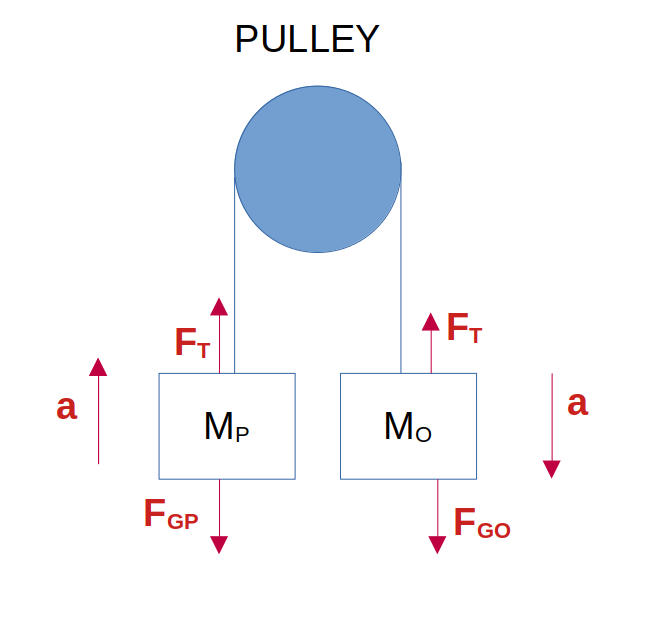
\includegraphics[scale=0.45]{atwood.png}
\caption{Concept Design - Atwood Machine}
\label{fig:atwood}
\end{figure}
A simple way to apply a known force can be realized through a basic pulley configuration known as an 'Atwood Machine.'\cite{monteiro2015atwood} As depicted in figure \ref{fig:atwood}, The only forces acting on the masses in the system are the gravitational force and tension(with the pulley assumed to be massless and frictionless).


\pagebreak
\bibliographystyle{IEEEtran}
\bibliography{ref}
\pagebreak

\appendices
\section{Experiment: Determination of the Range for the scale}\label{AppRange}
\subsection{Introduction}
The purpose of this experiment is to determine the range of the scale. This gives the user a sense of what range the scale is capable of measuring a reasonable mass.  

\end{document}
